\chapter{Platform}
\label{chap:platform}

In chapter \ref{chap:intro}, I explained the motivations behind the
Custos. Chapter \ref{chap:purpose} outlines the design goals and
potential applications that these motivations suggest. In this
chapter, I'll discuss the architecture, interface, and implementation
of Custos platform.

\section{Architecture}

The Custos architecture contains several core components:

\begin{packed_item}
\item A standardized API and message exchange format promoting the
  creation and proliferation of multiple implementations across a
  selection of providers.
\item A flexible server-side authentication interface, supporting an
  extensible variety of authentication attributes.
\item A programable server-side access control system for associating
  authenticated attributes with key:value access rights on a per-key
  basis.
\item A server-side back-end key:value store for holding persistent
  user and implementation data
\item A server-side data system for storing and retrieving user data
\item A server-side auditing system for monitoring and recording
  key:value access and authentication attempt data.
\item A server-side management system for configuring and controlling
  the other components.
\item One or more client applications that offload encryption keys or
  other secrets to a Custos server for storage and access control.
\end{packed_item}

\begin{figure}[!tb]
  \vspace{5ex}
  \begin{center}
    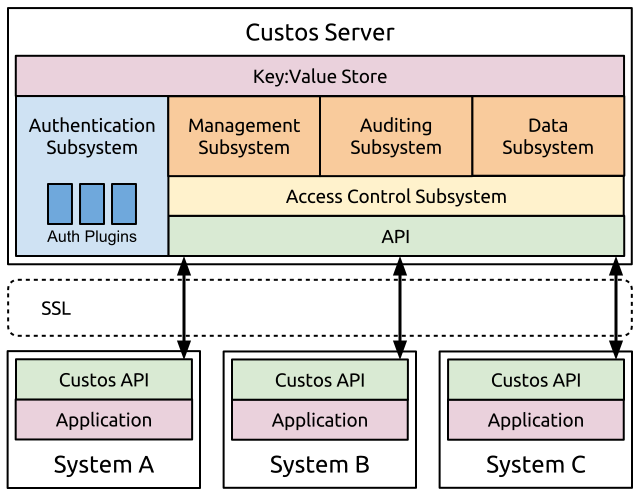
\includegraphics[width=.75\textwidth]
                    {./figs/pdf/Arch-Overview.pdf}
  \end{center}
  \caption{Basic Components of the Custos Architecture}
  \label{fig:arch-overview}
\end{figure}

Figure \ref{fig:arch-overview} shows the core Custos components. I'll
discuss the details of the Custos architecture in more details below.

The bulk of core Custos functionality is handled on the server
side. The server is designed to expose a single standardized API in
order to allow for a variety of inter-compatible implementations (one
possible implementation is discussed below). The Custos server
implements the following components:

\begin{packed_desc}
\item[API] \hfill \\ The server API handles all Custos requests,
  including requests for key:value data, requests to audit data
  access, and requests to modify data access controls. The API is
  essentially an RPC interface to allow applications to make requests
  of the Custos service.
\item[Access Control Subsystem] \hfill \\ The access control subsystem
  is the first step in the request processing pipeline after the
  API. The access control system compares the provided authentication
  attributes (calling into the authentication subsystem to verify
  them) to the set of required authentication attributes to determine
  if a Custos request should be allowed or denied.
\item[Authentication Subsystem] \hfill \\ The authentication
  subsystem's job is to verify the validity of any authentication
  attributes associated with a given Custos request. This subsystem is
  designed to allow for a pluggable authentication module interface
  capable of supporting a variety of authentication attributes.
\item[Data Subsystem] \hfill \\ The data subsystem is responsible for
  handling verified and accepted Custos data API requests (get, set,
  create, and delete key:value pairs). It interfaces with Key-Value
  store on one side and the access control system on the other.
\item[Auditing Subsystem] \hfill \\ The auditing subsystem is
  responsible for handling verified and accepted Custos audit API
  requests. The auditing subsystem is also concerned with logging all
  Custos requests and their corresponding responses. This data can
  then be used to generate reports related to the 'who', 'what', and
  'why' questions: \emph{Who} accessed (or failed to access)
  \emph{what} Custos stored data and \emph{why} where they granted or
  denied access (e.g. what authentication attributes did they present
  and were able to verify).
\item[Management Subsystem] \hfill \\ The management subsystem is
  responsible for handling all management related API requests after
  they have passed the authentication and access control layers. This
  primarily entails manipulating access control parameters.
\item[Key-Value Store] \hfill \\ The Key-Value store is the persistent
  data container associated with a given Custos server. It is used to
  store both end-user key:value pairs (encryption keys, etc) as well
  as a variety of internal Custos state (access control requirements,
  etc).
\end{packed_desc}

A Custos client applications interacts with a Custos server via the
API. As such, a client can simply offload the bulk of it's key
management directly to Custos through API-backed RPC libraries. Custos
simply becomes a remote key:value store where applications secrets are
stored. To satisfy Custos's authentication requirements, applications
can generate the necessary authentication attributes directly or can
instead pass these requirements on to the user, querying them for the
necessary attributes to send to Custos. Applications can either
implement their own auditing and management user controls directly,
passing the necessary information back to Custos via the API, or
applications can pass off auditing or management duties to separate
applications that interact directly with the Custos server.

\section{Access Control Abstraction}

As I already mentioned, the key:value abstraction Custos presents for
storing secrets is fairly well understood. It is Custos's access
control abstraction that is unique. This abstraction is at the core of
Custos's flexible capabilities.

\begin{figure}[!tb]
  \vspace{5ex}
  \begin{center}
    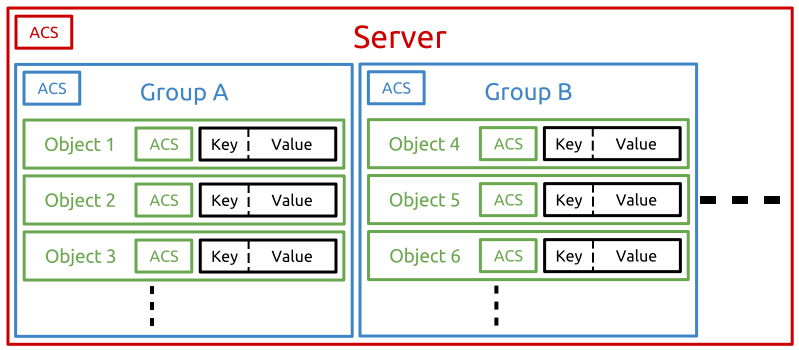
\includegraphics[width=.75\textwidth]
                    {./figs/pdf/Arch-OU.pdf}
  \end{center}
  \caption{Custos Organizational Units}
  \label{fig:arch-ou}
\end{figure}

In order to discuss the access control abstraction, I must first
explain the Custos \emph{organizational units} (OU). The Custos
architecture specifies three organizational units (Figure
\ref{fig:arch-ou}): a server, a group, and a key:value object. The
server unit is used to specify server-wide configuration. A server has
one or more groups. A group is used to slice a server between a
variety of administrative domains. It exists to allow a single server
to grant group-level administrative privileges to multiple,
non-cooperating entities (i.e. separate Custos provider customers). A
group, in turn, has any number of actual key:value objects stored
within it. Each OU is responsible for the creation of OU instances
beneath it, e.g. servers create groups and groups create objects.

\begin{figure}[!tb]
  \vspace{5ex}
  \begin{center}
    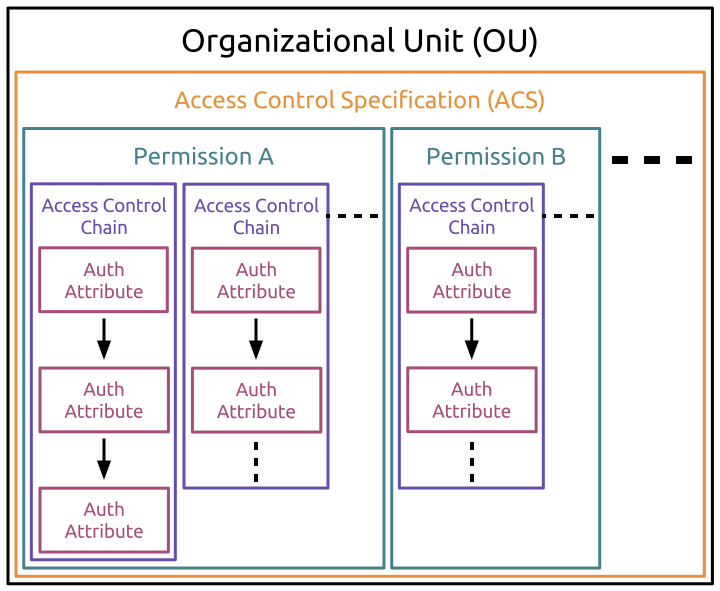
\includegraphics[width=.75\textwidth]
                    {./figs/pdf/Arch-ACS.pdf}
  \end{center}
  \caption{Custos Access Control Specification Components}
  \label{fig:arch-acs}
\end{figure}

The Custos access control abstraction revolves around designating an
\emph{Access Control Specification} (ACS) for each OU in the Custos
architecture. An ACS consists of three components (Figure
\ref{fig:arch-acs}). First, each ACS contains a full list of the
applicable Custos \emph{permissions} for the given OU. Associated with
each permission is one or more \emph{access control chains}
(ACCs). Each ACC in turn consist of an ordered list of
\emph{authentication attributes}.

\subsection{Permissions}

The Custos access control model starts with the concept of a
permission: a right to perform a specific Custos action. Custos has
specific permissions associated with each OU: per-server permissions,
each associated with the top-level Custos server, per-group
permission, each associated with a specific server group, and
per-object permissions, each associated with a specific key:value
object within a group.

Custos permissions are generally associated with the three core Custos
subsystems based upon the subsystem handling the associated actions
the permission grants: data access, auditing, and management. The
Custos data access permissions follow the pattern used by many data
access systems: permission to read data, permission to write data,
permission to create data, and permission to delete data. These
permissions are modified slightly to account for Custos's versioning
system. Unlike many system, Custos has no notion of object
ownership. Instead, it relies on providing access to each right an
owner would traditionally hold via explicit permissions. Likewise,
Custos associates audit permissions with various entities. Audit
permission grant read and delete access to various audit data.
Finally, the Custos management permissions control a users ability to
manage a specific Custos OU. This includes the ability to manipulate
OU access control specifications.

\noindent
The per-server (server-wide) Custos permissions are:

\begin{packed_desc}
\item[\texttt{srv\_grp}] \hfill \\ The \texttt{srv\_grp} permission
  grants a user the right to create, delete, or list groups on a
  Custos server. When created, this group is associated with an
  initial default ACS, programmable via the next two permission.
\item[\texttt{srv\_new\_grp\_acs\_get}] \hfill \\ The
  \texttt{srv\_new\_grp\_acs\_get} permission grants a user the right
    to read the default ACS applied to newly created groups.
\item[\texttt{srv\_new\_grp\_acs\_set}] \hfill \\ The
  \texttt{srv\_new\_grp\_acs\_set} permission grants a user the right
  to set the default ACS applied to newly created groups.
\item[\texttt{srv\_audit}] \hfill \\ The \texttt{srv\_audit}
  permission grants a user the right to read all audit information not
  associated with an existing server group. This includes information
  related to requests for non-existent groups, group creation, etc.
\item[\texttt{srv\_clean}] \hfill \\ The \texttt{srv\_clean}
  permission grants a user the right to delete all audit information
  not associated with an existing server group.
\item[\texttt{srv-acs-get}] \hfill \\ The \texttt{srv-acs-get}
  permission grants a user the right to view the per-server ACS
  controlling the permissions in this list.
\item[\texttt{srv-acs-set}] \hfill \\ The \texttt{srv-acs-set}
  permission grants a user the right to set the per-server ACS
  controlling the permissions in this list.
\end{packed_desc}

\noindent
The per-group (group-wide) Custos permissions are:

\begin{packed_desc}
\item[\texttt{grp\_obj}] \hfill \\ The \texttt{grp\_obj}
  permission grants a user the right to create, delete, or list
  key:value objects within a given group. When created, this object is
  associated with an initial default ACS, programmable via the next
  two permission.
\item[\texttt{grp\_new\_obj\_acs\_get}] \hfill \\ The
  \texttt{grp\_new\_obj\_acs\_get} permission grants a user the right
  to read the default ACS applied to newly created objects.
\item[\texttt{grp\_new\_obj\_acs\_set}] \hfill \\ The
  \texttt{grp\_new\_obj\_acs\_set} permission grants a user the right
  to set the default ACS applied to newly created objects.
\item[\texttt{grp\_audit}] \hfill \\ The \texttt{grp\_audit}
  permission grants a user the right to read all audit information not
  associated with an existing key:value object. This includes
  information related to requests for non-existent objects, object
  creation, etc.
\item[\texttt{grp\_clean}] \hfill \\ The \texttt{grp\_clean}
  permission grants a user the right to delete all audit information
  not associated with an existing key:value object.
\item[\texttt{grp\_acs\_get}] \hfill \\ The \texttt{grp\_acs\_get}
  permission grants a user the right to view the per-group ACS
  controlling the permissions in this list.
\item[\texttt{grp\_acs\_set}] \hfill \\ The \texttt{grp\_acs\_set}
  permission grants a user the right to set the per-group ACS
  controlling the permissions in this list.
\end{packed_desc}

\noindent
The per-object Custos permissions are:

\begin{packed_desc}
\item[\texttt{obj\_delete}] \hfill \\ The \texttt{obj\_delete}
  permission grants a user the right to delete all versions of an
  existing key:value object.
\item[\texttt{obj\_read}] \hfill \\ The \texttt{obj\_read} permission
  grants a user the right to read all versions of an exiting key:value
  object.
\item[\texttt{obj\_update}] \hfill \\ The \texttt{obj\_update}
  permission grants a user the right to create a new version of a
  key:value object. It is the Custos equivalent of a ``write''
  permission, but accounts for the fact the Custos key:value pairs are
  write-once objects, so ``writing'' to them really means creating a
  new version.
\item[\texttt{obj\_audit}] \hfill \\ The \texttt{obj\_audit}
  permission grants a user the right to read all audit information
  associated with an existing key:value object. This includes
  information related to object access (both granted and denied),
  object versioning, etc.
\item[\texttt{obj\_clean}] \hfill \\ The \texttt{obj\_clean}
  permission grants a user the right to delete all audit information
  associated with an existing key:value object.
\item[\texttt{obj\_acs\_get}] \hfill \\ The \texttt{obj\_acs\_get}
  permission grants a user the right to view the per-object ACS
  associated controlling the permissions in this list.
\item[\texttt{obj\_acs\_set}] \hfill \\ The \texttt{obj\_acs\_set}
  permission grants a user the right to set the per-object ACS
  associated controlling the permissions in this list.
\end{packed_desc}

\subsection{Access Control Chains}

Now that we've seen the available permissions contain in an ACS for a
specific OU, I can explain the next portion of an ACS: the access
control chains (ACCs). An access control chain is an ordered list or
authentication attributes. Each permission in an ACS is associated
with one or more ACCs. In order for a request to be granted a specific
permission, it must be bale to provide authentication attributes
satisfying at least one of the ACCs associated with that permission.

For example, consider a key:value object whose \texttt{obj\_read}
permission has the following ACC:

\begin{Verbatim}[samepage=true]
[ (username = 'Andy'), (password = '12345'), (src\_ip = 192.168.1.0/24) ]
\end{Verbatim}

In order for my read request for the associated key:value object to
succeed, I would have to make sure that my request contained all three
of the above authentication attributes. That would mean attaching the
'username' attribute to the request with a value of 'Andy', as well as
attaching the 'password' attribute to the request with a value of
'12345'. The src\_ip attribute is an implicit attribute (see next
section) and will be atomically added to my request when received by
the Custos server. In order to satisfy it, I would have to send the
request from the local network attached to the Custos server I'm
trying to query.

Looking at a slightly more complex example, consider the same
\texttt{obj\_read} permission, but this time with two separate ACCs
associated with it:

\begin{Verbatim}[samepage=true]
[ (username = 'Andy'), (password = '12345'), (src\_ip = 192.168.1.0/24) ]
[ (username = 'Andy'), (password = '12345'), (src\_ip = 75.148.118.216/29) ]
[ (username = 'John'), (password = 'Swordfish') ]
\end{Verbatim}

Now I am able to make the Custos request from either the local network
or from my home IP range. As long as I can satisfy at least one ACC in
a set of ACCs for a given permission, I am granted the right to
perform actions associated with the permission. I have also granted
access to an addition user, John, with his own password and no src\_ip
restriction.

This system is highly flexible. Take for example, the lack of explicit
username support anywhere in the Custos specification. As was done
above, usernames simply become another authentication attribute, often
the first attribute in a ACC to allow for all following attributes to
be made relative to the username attribute. But there's nothing
special about usernames. I could just have easily started each ACC
with a src\_ip, requiring a separate password based upon the location
a user is making their request from. The combination of simple ordered
attribute lists and a wide range of flexible attributes makes for a
very powerful access control system.

Another point worth noting is that sets of ACCs can be converted into
sets of trees, often simplifying the understanding of their
intent. ACC list sets are converted into ACC tree sets by combining
each attribute in matching attribute sub-lists across multiple lists
into single nodes in a ACC tree. For example, the previous set of ACC
lists could also be represented as:

\begin{center}
\begin{tikzpicture}
  \tikzset{level distance=30pt}
  \tikzset{sibling distance=0pt}
  \Tree [
    .\texttt{(username = 'Andy')}
    [ .\texttt{(password = '12345')}
      \texttt{(src\_ip = 192.168.1.0/24)} \texttt{(src\_ip = 75.148.118.216/29)} ]
  ]
\end{tikzpicture}
\begin{tikzpicture}
  \tikzset{level distance=60pt}
  \tikzset{sibling distance=0pt}
  \Tree [
    .\texttt{(username = 'John')}
    [ .\texttt{(password = 'Swordfish')} ]
  ]
\end{tikzpicture}
\end{center}

Finally, where desired, the Custos API can continue to prompt the user
for the next N missing attribute types in a chain. For now, N is a
per-implementation constant, but eventually N will be available as a
configuration parameter on a per-object basis. When N > 0, this
feature is leaking some authentication information in the form of the
required attribute types (although not their values), so it is left to
the user to decide when such leaking is acceptable and when it is
not. When in use, this feature allows a Custos server to engage in a
back-and forth with a client to prompt the client through all required
attribute types in an ACC. For example, in the case where N is equal
to 1, and the previously mentioned ACCs are in effect, the following
set of transactions would occur:

\begin{packed_enum}
\item The user sends a read object request with no attributes
\item The server respond that a username attribute is required
\item The user resubmits the request with an attached username
  attribute equal to 'Andy'
\item The server responds that a password is required
\item The user resubmits the response with a password equal to '12345'
\item As long as the user is submitting request from either the local
  network or my home IP range, the server will respond granting the
  request.
\end{packed_enum}

But what happens where there are multiple next steps in an ACC? For a
more complex request-response example, consider the ACC expressed in
the following tree:

\begin{center}
\begin{tikzpicture}
  \tikzset{level distance=60pt}
  \tikzset{sibling distance=0pt}
  \Tree [
    .\texttt{(username = 'Andy')}
    \texttt{(password = '12345')} \texttt{(auth\_cert = '0x32C59C00')}
  ]
\end{tikzpicture}
\end{center}

In this ACC, I must either provide a password or prove access to my
GPG authentication key. Rehashing the request-response sequence from
the previous ACC example:

\begin{packed_enum}
\item The user sends a read object request with no attributes
\item The server respond that a username attribute is required
\item The user resubmits the request with an attached username
  attribute equal to 'Andy'
\item The server responds that a password or a auth\_cert is required
\item The user resubmits the response with a password equal to '12345'
\item The server responds granting the request.
\end{packed_enum}

\subsection{Authentication Attributes}

Each Access Control Chain contains one or more Authentication
Attributes (AAs). An authentication attribute is a generic container
for authentication data. AAs contain the following information:

\begin{packed_desc}
\item[Class] \hfill \\ The class is the top level classification
  property of an AA. It is used to designate the nature of a given
  AA. Currently, Custos specific two possible values for class:
  ``implicit'' and ``explicit''. Implicit attributes are those that
  are automatically associated with a request (like an IP address or SSL
  client certificate). Explicit attributes are those that the user
  provides directly (like a password or token).
\item[Type] \hfill \\ Within a given class, the AA type specific which
  authentication plugin should handle a specific attribute. Details on
  currently supported Custos types are provided below.
\item[Value] \hfill \\ The value contains the arbitrary binary data
  associated with a given attribute. This could be a password, token,
  or portion of a handshake for more complicated authentication
  mechanisms.
\end{packed_desc}

The current Custos specification supports a handful of authentication
types. Thus far, the types support by Custos are primarily associated
with stateless authentication mechanisms. This simplifies the design
of the RESTful interface and authentication plugins. That said, Custos
eventually intends to supports fully arbitrary authentication
parameters, allowing authentication plugins to maintain their state
across requests where required. The currently defined implicit types
are:

\begin{packed_desc}
\item[\texttt{ip\_src}] \hfill \\ The source IP of a request as seen
  by the Custos server (e.g. the gateway IP is the source IP is behind
  a NAT device, etc). Compared against the required
  \texttt{$\langle$base$\rangle$/$\langle$mask$\rangle$} specification where
  included.
\item[\texttt{user\_agent}] \hfill \\ The HTTP user agent
  associated with a given request. Compared against the required text
  value where included.
\item[\texttt{auth\_type}] \hfill \\ The HTTP authentication type
  associated with a given request (i.e. none, basic, digest,
  tls). Compared against the required type where included.
\item[\texttt{auth\_value}] \hfill \\ The HTTP authentication value
  associated with a given request. Often a username or some other
  identifying value output by the HTTP servers internal authentication
  mechanisms. Compared against the required value where included.
\item[\texttt{time\_utc}] \hfill \\ The time the request arrived in
  UTC. Compared against the
  \texttt{$\langle$base$\rangle$/$\langle$mask$\rangle$} UTC time
  specification where included.
\end{packed_desc}

\noindent
The currently defined explicit types are:

\begin{packed_desc}
\item[\texttt{user\_id}] \hfill \\ An arbitrary value. Directly
  compared agings the required attribute value where included. Behaves
  the same as the \texttt{psk} type, but gets its own type for
  readability of semantic intent.
\item[\texttt{psk}] \hfill \\ An arbitrary value. Directly
  compared against the required attribute value where included.
\item[\texttt{psk\_sha256}] \hfill \\ An arbitrary value. Hashed with
  the sha256 algorithm with the result compared against the the
  required attribute value where included. Specifications related to
  iterations and salting are specified on a per-site basis.
\item[\texttt{psk\_bcrypt}] \hfill \\ An arbitrary value. Hashed with
  the bcrypt algorithm with the result compared against the the
  required attribute value where included. Specifications related to
  work factor and salting are specified on a per-site basis.
\end{packed_desc}

Other authentication types will be added as Custos matures. It's also
possible for Custos implementations to support non-standard types, but
this may effect inter-implementation compatibility. Implementations
that do use their own types may wish to propose them as official types
so that other implementations will support them as well.

\subsection{Example}

As an example showing the full access control process, consider a
Custos-backed encrypted file system application. Figure
\ref{fig:arch-request} shows two users of this application attempting
to access an encrypted file. In order to decrypt the file and provide
access, the encrypted file system must query Custos for the necessary
encryption keys.

\begin{figure}[!tb]
  \vspace{5ex}
  \begin{center}
    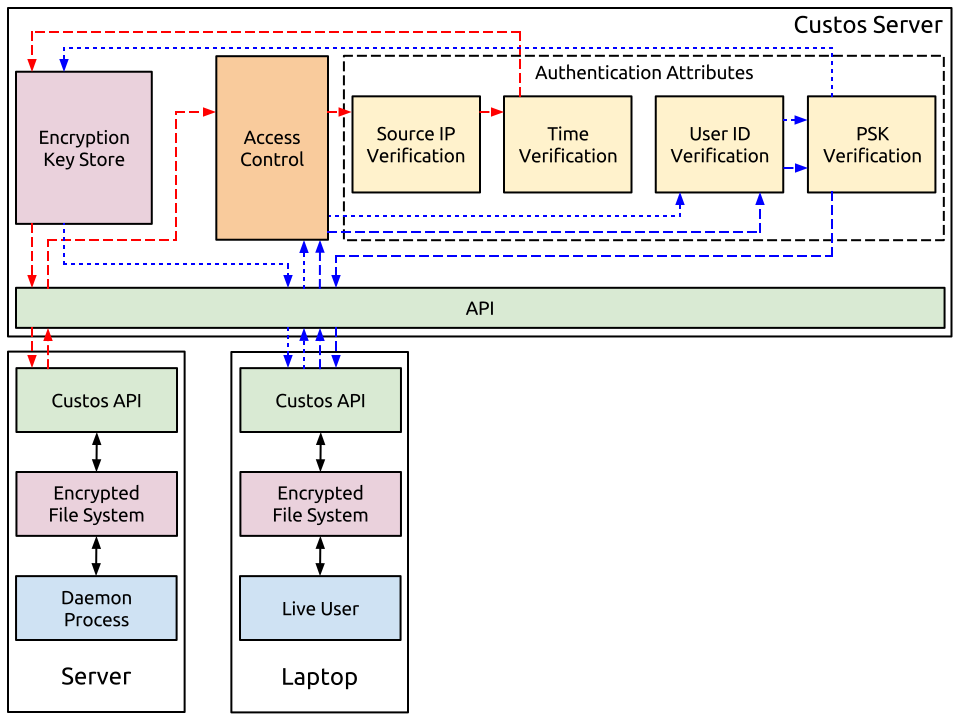
\includegraphics[width=.75\textwidth]
                    {./figs/pdf/Arch-KeyRequest-All.pdf}
  \end{center}
  \caption{An Example Custos Request Sequence}
  \label{fig:arch-request}
\end{figure}

The first user (red) is a daemon process running on a headless server
(IP = 1.2.3.4). The file the daemon wishes to read has an ACS
associated with it that contains the \texttt{obj\_read} permission and
grants access to this permission on the basis of the host IP and the
time:

\begin{Verbatim}[samepage=true]
{
  obj\_read:
    [
      [ (ip\_src = '1.2.3.4'), (time\_utc = '1300 +/- 5') ]
      ...
    ]
  ...
}
\end{Verbatim}

When the daemon reads the file, the encrypted file system requests the
associated encryption key from the server (dashed red line). The
request passes through the access control module, which looks up the
Access Control Chains associated with obj\_read permission for the
requested key:value pair. The requests is then passed to each of the
necessary Authentication Attribute modules in the order they appear in
the chain. Because the request is coming from an allows IP, it passes
the source IP verification module. Next, as long as the request is
being made within 5 minutes of 1300 hours UTC, the request will also
pass the time verification module. After satisfying both attributes
specified in the ACC, the request is granted the obj\_read permission
and passed to the audit module for logging. Finally, the server looks
up the requested key:value pair (in this case the encryption key for
the corresponding file) in the key:value store, generates a response,
and returns it to the encrypted file system. The file system decrypts
the file and returns it to the daemon that originally made the read
request. All of this is done without any interactive input on the part
of the daemon, overcoming one of the traditional obstacles to using
encryption with automated processed.

The second user (blue) is a live user named Dirk also trying to read a
file on the encrypted file system. The file the user wishes to read
has an ACS associated with it that contains the \texttt{obj\_read}
permission and grants access to this permission on the basis of the
user ID and a password:

\begin{verbatim}
{
  obj\_read:
    [
      [ (user\_id = 'Dirk'), (psk = 'WorldOfBeer') ]
      ...
    ]
  ...
}
\end{verbatim}

When user reads the file, the encrypted file system requests the
associated encryption key from the server (dashed blue line),
attaching the current users ID of 'Dirk' to the request (but excluding
the password). The request passes through the access control module,
which, as before, looks up the Access Control Chains associated with
the obj\_read permission for the requested key:value pair. The request
is then passed to the user ID verification authentication plugin,
which confirms that the user ID of Dirk is present, next the request
is passed to the PSK module for password verification. Unfortunately,
the request lacks the necessary password, so the server responds to
the request informing the encrypted file system that a password is
required for user 'Dirk'. The encrypted file system prompts the user
for their password, and reissues the request, including everything
from the first request and in addition the newly provided password
(dotted blue line). This time the request clears both AA verification
modules, passes through the auditing system, and finally hits the
actual key:value store. Here the server looks up the requested key,
generates a response, and returns it to the file system. The file
system decrypts the requested file and allows the user's read to
proceed on the resulting clear text.

\section{API}

The Custos API is the primary interface for interacting with a Custos
server. The API handles, data, management, and auditing requests
through a common interface. All API requests can contain
authentication attributes as a means of attaining the necessary
permission level for a requested operation. The API is RESTful and
primarily stateless (individual authentication modules are allowed to
maintain state if required).

API requests are made to specific server HTTP endpoints. The standard
HTTP verbs (\texttt{GET}, \texttt{POST}, \texttt{DELETE}, etc) are
used to multiplex related operations atop a specific endpoint. Each
combination of endpoint and verb defines a specific API method. Each
method required specific permission to complete. The API request and
response message formats are composed in JSON. Binary data is encoded
as Base64 ASCII text. When made as a \texttt{GET} request using a
query string, JSON messages are URL encoded.

\subsection{Message Format}

API requests and response use standard JSON objects as the basis for
their message formats. Each request or response message shares a
standard format. The effect of the message is determined by it's
contents, as well as the endpoint and verb user to send it to the
server. Examples API messages can be found in Appendix
\ref{appx:messages}.

The following are the required components in any Custos message. Each
is represented as a key:value pair in the top level JSON message
object.

\begin{packed_desc}
\item[\texttt{Version}] \hfill \\ The Custos protocol version. Used to
  determine server compatibility with a given Custos message format
  and method semantics.
\item[\texttt{Group}] \hfill \\ A UUID uniquely identifying the group
  associated with the message. If left blank, the message is assumed
  to apply at a server-wide level.
\item[\texttt{ReqID}] \hfill \\ A UUID uniquely identifying the
  request message (or the request message that triggered the response
  message).
\item[\texttt{ResID} (Response Only)] \hfill \\ A UUID uniquely
  identifying the response message.
\item[\texttt{Status} (Response Only)] \hfill \\ The status of the
  response. Used to indicate errors processing the corresponding
  request (malformed request, etc).
\item[\texttt{Attrs}] \hfill \\ A list of Custos \texttt{Attrs}. Used
  to identify or provide the AAs associated with the message.
\end{packed_desc}

Furthermore, each message may cont in one or more of the following
optional components:

\begin{packed_desc}
\item[\texttt{Keys}] \hfill \\ A list of Custos \texttt{Key}
  objects. Used to identify or provide the key:value objects a
  associated with the message.
\item[\texttt{ACSs}] \hfill \\ A list of Custos \texttt{ACS}
  objects. Used to provide the ACS associated with the message.
\end{packed_desc}

\noindent
Custos \texttt{Attr} objects have the following components:

\begin{packed_desc}
\item[\texttt{Class}] \hfill \\ The AA class
\item[\texttt{Type}] \hfill \\ The AA type
\item[\texttt{Value}] \hfill \\ The AA value, encoded as Base64 ASCII.
\item[\texttt{Echo}] \hfill \\ A Boolean indicting whether or not the
  server should (when possible) echo the value of the \texttt{Attr}
  contained in a request back to the user in the response.
\item[\texttt{Status} (Response Only)] \hfill \\ The status indicating
  whether a given AA was accepted, denied, ignored, or required.
\item[\texttt{ResValue} (Response Only)] \hfill \\ An arbitrary
  response from a given AA module providing details on the nature of
  the status or instructions on how to continue. Encoded as Base64
  ASCII.
\end{packed_desc}

\noindent
Custos \texttt{Key} objects have the following components:

\begin{packed_desc}
\item[\texttt{UUID}] \hfill \\ The UUID identifying the key
\item[\texttt{Revision}] \hfill \\ Used to request a specific key
  revision. If blank, the latest revision is assumed.
\item[\texttt{Value}] \hfill \\ The corresponding value, encoded as
  Base64 ASCII. May be left blank (e.g. as in read requests where its
  value is unknown).
\item[\texttt{Echo}] \hfill \\ A Boolean indicating whether or not the
  server should (when possible) echo the value of the \texttt{Key}
  contained in a request back to the user in the response.
\item[\texttt{Status} (Response Only)] \hfill \\ The status indicating
  whether the requested operation on the Key was allowed or denied.
\end{packed_desc}

\noindent
Custos \texttt{ACS} objects have the following components:

\begin{packed_desc}
\item[\texttt{Permissions}] \hfill \\ A dictionary of Permission:(ACC
  list) pairs. Each ACC list is, in turn a list of Attr objects
\item[\texttt{Echo}] \hfill \\ A Boolean indicating whether or not the
  server should (when possible) echo the value of the \texttt{ACS}
  contained in a request back to the user in the response.
\item[\texttt{Status} (Response Only)] \hfill \\ The status indicating
  whether the requested operation on the ACS was allowed or denied.
\end{packed_desc}

\subsection{Endpoints}

Data:

objs - create, read, update, del
grps - create, list, del

Management:

obj\_acs - get, set
new\_obj\_acs - get, set
grp\_acs - get, set
new\_grp\_acs - get, set
srv\_acs - get, set

Auditing:

obj\_audit - get, clean
grp\_audit - get, clean
srv\_audit - get, clean

\section{Prototype Implementation}

\subsection{API}

JSON RESTful API

\subsection{Authentication and Access Control}

Standardized module interface

\subsection{Back-end Storage}

Variable back-end key-value providers

%%  LocalWords:  ACS ACCs ACC OU srv grp src ip usernames auth acs
%%  LocalWords:  username AAs tls psk sha bcrypt utc del ReqID ResID
%%  LocalWords:  Attrs ACSs Attr ResValue
